\title{Final year project}
\author{
        Leonardo Ciocan
}
\date{\today}

\documentclass[12pt]{article}
\usepackage{titlesec}
\usepackage{setspace}
\usepackage{graphicx}
\usepackage{float}% If comment this, figure moves to Page 2


\titleformat*{\section}{\LARGE\bfseries}

\begin{document}
\maketitle

\clearpage

\begin{abstract}
In university settings, lecturers often teach classes of up to 200 students. Often they distribute papers to gauge the student’s understanding of the current material being taught. The distribution, collection and analysis of these materials makes it hard for the lecturer to evaluate which parts of the material the students need help with.
I have created a digital solution that helps the teacher get a better understanding of his students progress in real time.

\end{abstract}
\clearpage

\doublespacing
\tableofcontents
\singlespacing
\clearpage



\section{Introduction}
\subsection{Summary}
There is quite a sizeable market that would benefit from this application, there are 23729 universities around the world; a high percentage of them have Computer Science departments.
Competitors
Some companies have products that aim to facilitate teacher – student interaction but I believe they are rather incomplete and further more none appear to provide tools specifically for computer science students. In other words, they provide generic tools for letting students answer questions but that is not tailor for computer science specifically.
Motivation
The main scope of my project was to create an easily extensible platform that may be useful for teachers specifically teaching computer science as this subject in particular requires some types of question that are more complex than simple text or choices. In other words, letting users write and execute code on my platform was a core goal. Executing arbitrary code is a dangerous so security is an important part of this system.
This project is a great way to experiment with visualisation of data and how digital solutions can enrich previous analogue methods , it also allowed me to work with technologies I had not worked before and build a full product which enriched my knowledge of security , containers , server and backend technologies.

\subsection{Report structure}
The next section will be the background which will begin by exploring the keywords or concepts that are related to the project.
It will also analyse and contrast current implementation that attempt to solve the problem described with the project's implementation.

\subsection{Platform}
I have decided to build this project for the web instead of a mobile application for a number of reasons. Since this is meant to be used by a lot of students, it is a requirement that it should be as accessible as possible. Statistically speaking, a web app can reach the most people, especially account for the fact that computing students are the main target audience and they are likely to have laptops with them.
The main disadvantage of making mobile apps is that to build a good native app would mean to focus on one platform (as cross platform solutions are not up to the task for the scope of the project) which would exclude students from the process. The web is a free, universal platform and so it is the perfect medium for this project.
Ideally, fully native mobile apps are further down the roadmap as they provide a better experience and further expand the pool of users that are able to use the application.
The backend part of this project has been built in such a way to allow for easy expansion to other platforms. In fact, the web app could be considered just a consumer of the backend and not being renderer by the server such that another front-end could be used instead without any friction.



\subsection{Objectives}
Because the main target audience is made up of computer savvy student and lecturers, it was possible to take a few liberties with the platform. For example the questions can be written in Markdown, which is something computer scientists are already familiar with from websites such as StackOverflow and Github.
Nevertheless, I aim to make a project that requires minimal guidance as the user interface will be built to be easy and intuitive to operate.

The basic requirements for this project are:
\begin{enumerate}
\item Let teacher create sheets made of a variety of question types
\item 	Allow question types to include rich formatting such as tables and code
\item 	Allow students to subscribe to a lecture such that they may have access to those sheets
\item 	Allow a teacher to create a class and invite students with a link
\item 	Let the teacher decide when a sheet should go “live” and be visible by the students
\item 	Allow the teacher to attach model answers to each question
\item Let the teacher release model answers to the students so they may review their answers
\item 	Monitor the students progress and present it to the teacher in an anonymous way
Allow users to write code to be executed for code questions

\end{enumerate}

\section{Background}
\subsection{Relevant concepts}
\paragraph{Question}
Currently there are 3 types of questions:
\begin{itemize}
\item Multiple choice: The user is presented some choice and selects one
\item Input: The user may input any piece of text, multiple solutions can exist
\item Code: Users can write code to solve a posed question
\end{itemize}

The system is built in such a way that adding further questions is trivial and does not require breaking backwards compatibility or redesigning data structures used on the server.

\paragraph{Sheet}
The application revolves around Sheets. Analogue to a paper sheet handed in class, a sheet is a collection of questions of various types. Each sheet belongs to a lecture which has a teacher.


A teacher can create sheets by mix and matching any number of question types which enable quite a varied way to test their students.

\paragraph{Lecture}
A lecture is a collection of sheets. It has a teacher and students can subscribe to a lecture so they can have access to all the sheets.
Dashboard
An important part of this project is for the teacher to be able to monitor the student progress so that they may respond accordingly (for example, write some hints on the board). Each sheet has a dashboard which only the teacher can access.
For each type of question, there is a different specialised user interface that is tailored to convey the progress of the students.
A code question's dashboard widget will show the percentage of students who completed the question. 
An input question’s dashboard shows the percentage of completions, as well as a word cloud of popular words in the questions, this is a specialised control that visually conveys to the teacher common words that are being used.
A choice question’s dashboard will show the user’s completion, a bar chart for top first choices (which could help identify misleading questions amongst other things) and a transition matrix table, which shows the way students move from one answer to another.

The dashboard is also meant to be extensible, so any future question types could provide their own way of visualising student progress.

\subsection{Differentiation from competitors}
The project is meant to be an extensible platform that can be enriched with more types of question along the development process to increase the variety of sheets the teachers can create. This gives it more potential than competitor’s who over inflexible solutions that are tailor made for very specific types of questions.
Furthermore, by focusing on computer science students we allow users to run arbitrary code on the platform, which while some websites allow that – they provide that in a different setting such as code competitions – which means they do not compete with us , as this project enabled the teacher to write a question that can be answered with code as part of a sheet along with other questions.

\subsection{Security}
Because the project allows users to input and run arbitrary code it is important to have proper security in place. There are three layers of security for running code:
\begin{itemize}
\item Users can only run non-native code , currently Python and Java
\item 	All user code runs in secure Docker containers
\item	All containers are contained in a separate server
\end{itemize}
Because the code execution server and the database/main server are separate – even if a malicious agent used a vulnerability to break out of the container, he may not access any information or maliciously disrupt server operations.

//security stats about safe code


\section{Requirements}
\section{Design}
This section will present an abstract view of how the system works.

\subsection{Use cases}
\begin{figure}[H]
  \centering

	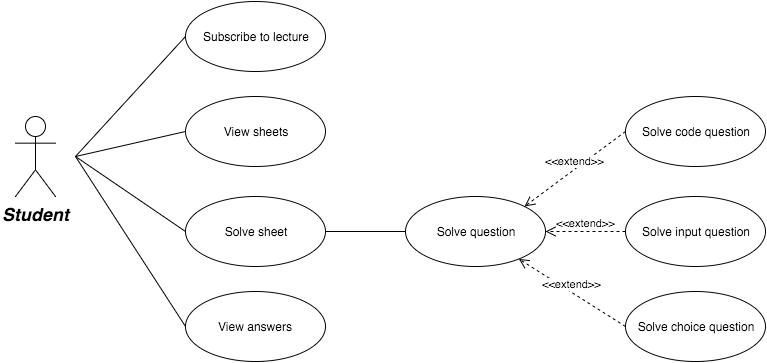
\includegraphics[width=\textwidth,height=\textheight,keepaspectratio]{cases}
	\caption{Use cases for students}
\end{figure}

\begin{figure}[H]
  \centering

	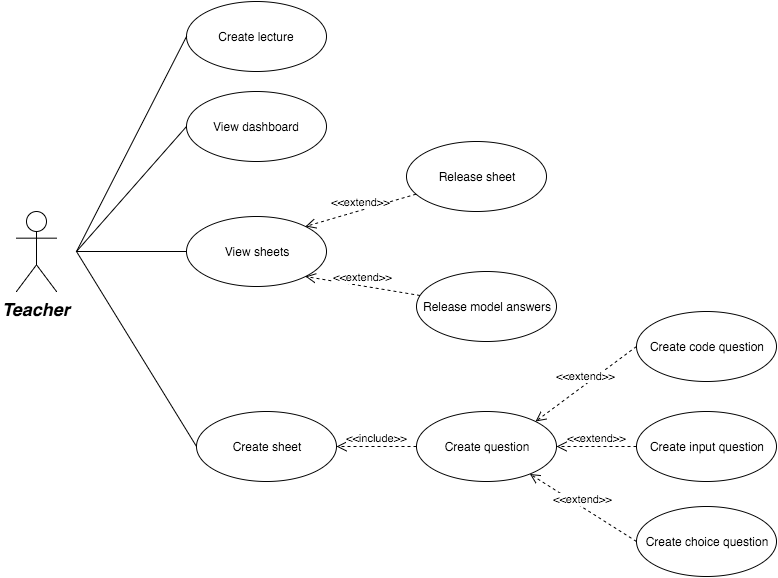
\includegraphics[width=\textwidth,height=\textheight,keepaspectratio]{cases2}
	\caption{Use cases for teachers}
\end{figure}

\subsection{System architecture}
\paragraph{User interface}
Since the user's are assumed to be somewhat technically savvy , the application takes some liberties with having a limited amount of help and information banners since it works similarly to other website the target audience is familiar with.
Overall the application is meant to have a flat design that looks good on any resolution.
Each lecture has a colour chosen by the teacher and shows up throughout the user interface so the user knows which lecture they are looking at.

\subsection{Third party libraries}

\subsubsection{React}
A javascript library that allows the project to have isolated , reusable components that build up all of the user interface

\subsubsection{Chromath} 
A javascript library that can manipulate colours. It is used within the dashboard to compute darker shades of the lecture color - this is useful for both the charts ( each section of the chart is a different colour ) and for the transition matrix ( the higher the transition count , the darker the shade ).

	It is statically included in the project.
	
\subsubsection{CodeMirror}
A javascript library that provides an embeddable code editor. Used to let user's write their own code.

\subsubsection{Markdown-it}
A javascript library used to render Markdown , in both the title preview on the sheet creation page and the actual sheet that the user sees.

\subsubsection{Highlight}
A javascript library to highlight code syntax , used internally by Markdown-it
	
\subsubsection{JQCloud}
A javascript library used to render a word cloud in the dashboard for input questions.

\subsubsection{Levenshtein-ffi}
A ruby gem that allows fast calculation of Levenshtein distances for answer's in the input question's dashboard.

\subsubsection{pg}
A ruby gem for Postgres support

\subsubsection{Devise}
A ruby gem that simplifies authentication

\subsubsection{ReactRails}
Support for React in Rails applications

\subsubsection{Typescript Rails}
Automatic compilation of typescript files as part of the rails asset pipeline.


\section{Implementation and Testing}

\subsection{Unit testing}
Unit testing was used to make sure changes and additions to the system did not break or alter any previous functionality.

Purpose:
\begin{enumerate}
	\item To make sure existing functionality was not compromised
	\item To ensure that the database settings worked as intended ( defaults , uniqueness etc)
	\item Components of the system all complied with security , such as preventing user's from editing other people's date or gaining access to data they are not allowed to see
\end{enumerate}


\section{Professional Issues}

\section{Evaluation}
In this section we will explore whether the project has met the requirements that were set in the requirements section of this report as well as other general aspects of the software that can be evaluated.

\subsection{Limitations}
There were some things that were simplified or postponed for the sake of keeping in line with deadlines and achieving all the compulsory requirements that I have set. Thus the system does have some limitation (solutions to those limitations will be explored in the next section)

\begin{itemize}
	\item Code question can be either Java or Python based. This is a limitation imposed to decrease the surface area for bugs that would arise from allowing more languages.
	\item Sheets cannot be edited after they are created. This is because changing the questions as the sheet is live could invalidate existing statistical data retrieved from users completing the question.
	\item Teacher cannot kick out or manage users. This is because currently the system aims to anonymise users so they may not feel discouraged from completing the questions
	\item The website is glitchy and may not work at all on some mobile devices. This is especially true for pages where the user may enter a core
\end{itemize}

\subsection{Security}
While the system is not meant to contain any sensitive data , it is important that the users of the system can be assured that their data is private. 
There are safeguards in place to ensure that a malicious agent may not successfully acquire information they are not entitled to , this functionality is unit tested to ensure it stays this way across releases of the software.
Another layer of security is in the system that executes the student's arbitrary code.
The code runs in a docker container and can only run within either the java virtual machine or the python interpreter. Not allowing low level code to run discourages any traditional security holes such as buffer overflows.
Furthermore , even if someone manages to execute code such that they break out of the language runtime and the docker container - the containers run on a server separate from the main server. Thus they cannot access the database or compromise the system.

\subsection{Overall}
The main purpose of the system was to provide teacher's a way to handle handing out sheets digitally and analyse the result easily in real time. It was built in such a way that not only fulfilled this requirement but also provides a platform that is easily extendable such that more question types can be added without having to modify the existing infrastructure.



\section{Conclusion and future work}

\subsubsection{Future work}
There are a number of ways to improve the project , the system is implemented in such a way that adding more functionality can be done seamlessly without breaking or having to alter any major components of the system.

Ideas for improvements:
\begin{itemize}
	\item More question types. For example questions that revolve around web development ( such as asking the user to create a html/css layout from an image) or unix command line tools ( asking the user to complete some command line workflow ). This should be easy to implement as the database schema for questions is very flexible and does not make any assumptions about the type of data a question expresses
	\item Better user management for the teacher , allowing them to kick , filter and analyse student progress. This would involve adding a lot more UI components and possibly other pages
	\item Allowing teacher to edit the title/body of questions after the sheet is created. Easy to implement the technical aspect of it , however it would not fit within any current place in the UI and would require an additional page
	\item Password enabled lectures , or alternatively geo-locked lectures. Fairly simple to implement but needs to have extra logic in place to deal with changing the password and so on
	\item Mobile apps for Android and iOS to expand the pool of students who have a device that can use the project. Takes time but overall the backend would not have to be changed much as it already exposes most functionality via a simple REST API
\end{itemize}


\section{Definitions}
Here is a list of words that may be useful in reading this report:

\paragraph{Question} A computable question that is posed to the user

\paragraph{Input Question} A question where the user can enter any text in a text box , the solution is expressed by a regex

\paragraph{Choice Question} A question where the user can chose one item from a predefined set

\paragraph{Code Question} A question where the user can answer by writing a piece of code

\paragraph{Sheet} A collection of questions

\paragraph{Lecture} A collection of sheets that students may subscribe to

\paragraph{UI} User Interface , describes what the users sees and interacts with

\paragraph{REST API} An interface that the server exposes that allows the client to interact with the service over standard HTTP requests

 



















\end{document}